\documentclass[a4paper,fleqn]{cas-dc}

% If the frontmatter runs over more than one page
% use the longmktitle option.

%\documentclass[a4paper,fleqn,longmktitle]{cas-dc}

\usepackage[numbers]{natbib}
%\usepackage[authoryear]{natbib}
%\usepackage[authoryear,longnamesfirst]{natbib}

%%%Author macros
\def\tsc#1{\csdef{#1}{\textsc{\lowercase{#1}}\xspace}}
\tsc{WGM}
\tsc{QE}
%%%

% Uncomment and use as if needed
%\newtheorem{theorem}{Theorem}
%\newtheorem{lemma}[theorem]{Lemma}
%\newdefinition{rmk}{Remark}
%\newproof{pf}{Proof}
%\newproof{pot}{Proof of Theorem \ref{thm}}

\begin{document}
\let\WriteBookmarks\relax
\def\floatpagepagefraction{1}
\def\textpagefraction{.001}

% Short title
\shorttitle{short title}

% Short author
\shortauthors{O. Olikh}

% Main title of the paper
\title [mode = title]{main title}

% First author
%
% Options: Use if required
% eg: \author[1,3]{Author Name}[type=editor,
%       style=chinese,
%       auid=000,
%       bioid=1,
%       prefix=Sir,
%       orcid=0000-0000-0000-0000,
%       facebook=<facebook id>,
%       twitter=<twitter id>,
%       linkedin=<linkedin id>,
%       gplus=<gplus id>]
\author{Oleg~Olikh}
%\cormark[1]
\ead{olegolikh@knu.ua}
%\address[1]{Taras Shevchenko National University of Kyiv, 64/13, Volodymyrska Street, City of Kyiv, Ukraine, 01601}


% Address/affiliation
\affiliation{organization={Taras Shevchenko National University of Kyiv},
            addressline={64/13, Volodymyrska Street},
            city={Kyiv},
%          citysep={}, % Uncomment if no comma needed between city and postcode
            postcode={01601},
 %           state={},
            country={Ukraine}}

% For a title note without a number/mark
%\nonumnote{}

% Here goes the abstract
\begin{abstract}
Defect-assisted recombination processes frequently
limit the photovoltaic device performance.
The low-cost and express methods of impurity contamination control
are in demand at solar cell manufacturing.
In this paper, we applied deep learning-based
approach to extract the iron concentration in silicon solar cell from an
ideality factor values.
\end{abstract}

% Use if graphical abstract is present
%\begin{graphicalabstract}
%\includegraphics{}
%\end{graphicalabstract}

% Research highlights
\begin{highlights}
\item Proposed deep learning-based method to predict iron contamination in Si-SC by using IV curve.
\item The simulated IV characteristics are used to create training and test datasets.
\item The DNN's configurations are proposed.
\item The mean squared relative error of prediction is up to 0.005.
\end{highlights}

% Keywords
% Each keyword is seperated by \sep
\begin{keywords}
Ideality factor \sep Silicon \sep $n^+$--$p$--$p^+$ structure \sep
SCAPS \sep Iron contamination \sep Machine learning
\end{keywords}

\maketitle

% Main text
\section{Introduction}\label{}


\section{Solar cell model}\label{}
Fig.~\ref{fig_chem}
vividly reveals the structure of the used model \cite{Castro2010}. 
It can be seen from the figure that model contains a current source accompanied by a diode D1, a shunt
resistor $R_\mathrm{p1}$ to show the leakage current, and a series resistor $R_\mathrm{s}$ to consider the
losses associated with the load current.
Besides, the second diode D2 with a second parallel resistance $R_\mathrm{p2}$ is placed opposite to the first one and is essential to
simulate the non-ideal effects of the active layer/cathode interface.
In this model, D1 is responsible for the exponential behavior of the I--V curve,
the main contribution of D2 is to simulate the S--shape.
The analytical solution $V(I)$ of the opposed two--diode equivalent circuit model was
 obtained \cite{CastroSolution} using Lambert $W$-function \cite{LambertNew}:


\begin{figure}[]
	\centering
		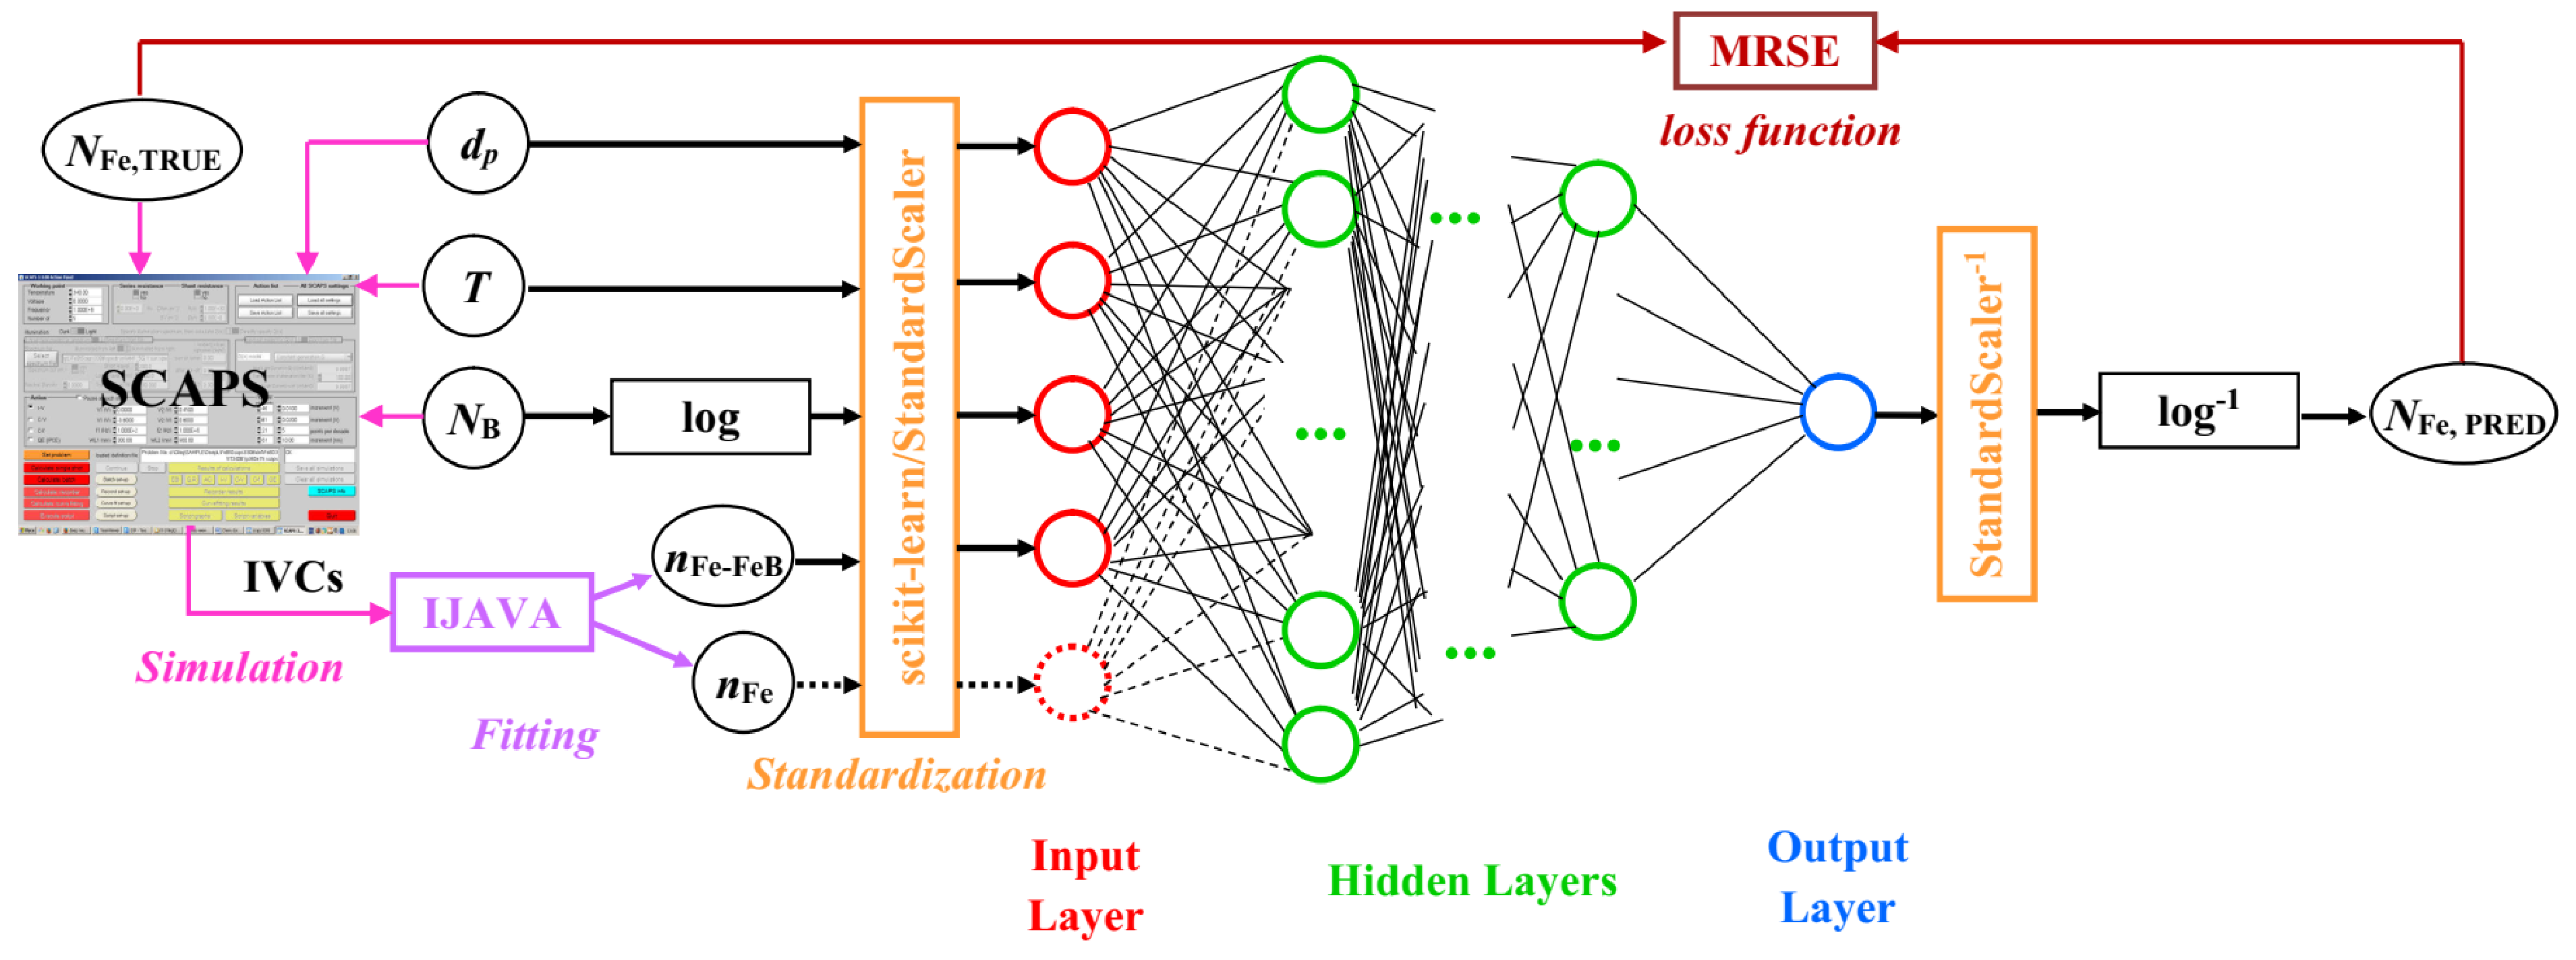
\includegraphics[width=0.9\columnwidth]{Chem}
	  \caption{The opposed two--diode equivalent--circuit model of a solar cell.}\label{fig_chem}
\end{figure}


\begin{eqnarray}
% \nonumber to remove numbering (before each equation)
\label{eqIV_W}
V&=& (I+I_\mathrm{ph}+I_{01})R_\mathrm{p1} \nonumber \\
  &&-\frac{n_1kT}{q}W\left\{\frac{qI_{01}R_\mathrm{p1}}{n_1kT}\exp\left[\frac{qR_\mathrm{p1}(I+I_\mathrm{ph}+I_{01})}{n_1kT}\right]\right\} \nonumber \\
  &&+\frac{n_2kT}{q}W\left\{\frac{qI_{02}R_\mathrm{p2}}{n_2kT}\exp\left[-\frac{qR_\mathrm{p2}(I-I_{02})}{n_2kT}\right]\right\} \nonumber \\
  &&+(I-I_{02})R_\mathrm{p2}+IR_\mathrm{s}\,,
\end{eqnarray}
where
$I_{01}$ and $I_{02}$ are the saturation currents and 
$n_1$ and $n_2$ are
the ideality factors for D1 and D2 respectively, 
and $I_\mathrm{ph}$ is the ideal photocurrent.
Thus, the model employs eight lumped parameters 
($I_{01}$, $n_1$, $R_\mathrm{p1}$, $I_{02}$, $n_2$, $R_\mathrm{p2}$,
$R_\mathrm{s}$, and $I_\mathrm{ph}$)
that need to be determined from the I-V curve.

The expression~(\ref{eqIV_W}) has a drawback in that it tends to stray from the range of numbers that can be accommodated by the standard 64-bit floating-point format owing to the presence of exponential functions for larger numbers.
To overcome this drawback, the use of the $g$--function $g(x)=\ln(W(\exp(x)))$ was suggested.




In our previous work, we have shown that the SC ideality factor value ($n$) can be used to estimate the iron concentration ($N_{\mathrm{Fe}}$).
It should be noted that the ideality factor is quite often  used to characterize the various
semiconductor barrier structures.
However, a defect's signature in an ideality factor is convoluted with those from so many other physical processes.
As a result, obtained analytic expressions $N_{\mathrm{Fe}}=f(n)$ are not general and the numerous grading curves are required to determine $N_{\mathrm{Fe}}$;
besides the IV measurements over a temperature range are necessary.
On the other hand, in the last decade, the deep learning, which enables to solve problems without clear algorithmization, have been successfully used in various fields of theoretical and applied physics.
Furthermore, materials informatics
(combination of material property calculations/measurements and informatics algorithms)
has been asserted to become the fourth (along with theory, simulations, and experiments) paradigm of science.
The aim of this work is to apply the deep learning approach for predicting of the iron concentration from ideality factor
(so to say "deep learning for deep levels").
Further, unlike in previous work, the back surface field (BSF) $n^+$--$p$--$p^+$ structure was under consideration
and the influence of the base thickness on ideality factor was taken into account as well.

As the approximation to the practical using, the paper considers a fairly simple system
which consists of crystalline silicon (c-Si) SC  and iron impurity.
However, the system is important in practice.
Silicon solar cells constitute ~90\% of current global production capacity and
BSF  is one of  popular designs used for industrial mass production of c-Si SCs .
Iron is a major as well as one of the most detrimental metallic impurities in c-Si SCs .
The flowchart of the used heuristic approach is shown in Fig.~\ref{fig_chem}.
The following constituents can be distinguished.
First, the dark IV characteristics are simulated for SCs with both known contaminant composition and various parameters.
In our numerical simulation we applied SCAPS-1D,
which widely used to model solar cells .
Second, the obtained characteristic is fitted according to the double-diode model and the ideality factor is estimated.
As a result of aforesaid steps, the labeled datasets were produced.
Obviously, the labeled dataset from experimental IVs  would be preferable,
but it is practically difficult to find the thousands of samples with the required parameters.
Third, the training of deep neural network (DNN) to estimate an iron contamination  by using SC's base thickness, doping level,
temperature, and ideality factor value.
Fours, the DNN testing.


% Numbered list
% Use the style of numbering in square brackets.
% If nothing is used, default style will be taken.
%\begin{enumerate}[a)]
%\item
%\item
%\item
%\end{enumerate}

% Unnumbered list
%\begin{itemize}
%\item
%\item
%\item
%\end{itemize}

% Description list
%\begin{description}
%\item[]
%\item[]
%\item[]
%\end{description}

% Figure
%\begin{figure}[<options>]
%	\centering
%		\includegraphics[<options>]{}
%	  \caption{}\label{fig1}
%\end{figure}


\begin{table}[<options>]
\caption{}\label{tbl1}
\begin{tabular*}{\tblwidth}{@{}LL@{}}
\toprule
  &  \\ % Table header row
\midrule
 & \\
 & \\
 & \\
 & \\
\bottomrule
\end{tabular*}
\end{table}

% Uncomment and use as the case may be
%\begin{theorem}
%\end{theorem}

% Uncomment and use as the case may be
%\begin{lemma}
%\end{lemma}

%% The Appendices part is started with the command \appendix;
%% appendix sections are then done as normal sections
%% \appendix

\section{}\label{}

In our previous work, we have shown that the SC ideality factor value ($n$) can be used to estimate the iron concentration ($N_{\mathrm{Fe}}$).
It should be noted that the ideality factor is quite often  used to characterize the various
semiconductor barrier structures.
However, a defect's signature in an ideality factor is convoluted with those from so many other physical processes.
As a result, obtained analytic expressions $N_{\mathrm{Fe}}=f(n)$ are not general and the numerous grading curves are required to determine $N_{\mathrm{Fe}}$;
besides the IV measurements over a temperature range are necessary.
On the other hand, in the last decade, the deep learning, which enables to solve problems without clear algorithmization, have been successfully used in various fields of theoretical and applied physics.
Furthermore, materials informatics
(combination of material property calculations/measurements and informatics algorithms)
has been asserted to become the fourth (along with theory, simulations, and experiments) paradigm of science.
The aim of this work is to apply the deep learning approach for predicting of the iron concentration from ideality factor
(so to say "deep learning for deep levels").
Further, unlike in previous work, the back surface field (BSF) $n^+$--$p$--$p^+$ structure was under consideration
and the influence of the base thickness on ideality factor was taken into account as well.

As the approximation to the practical using, the paper considers a fairly simple system
which consists of crystalline silicon (c-Si) SC  and iron impurity.
However, the system is important in practice.
Silicon solar cells constitute ~90\% of current global production capacity and
BSF  is one of  popular designs used for industrial mass production of c-Si SCs .
Iron is a major as well as one of the most detrimental metallic impurities in c-Si SCs .
The flowchart of the used heuristic approach is shown in Fig.~\ref{fig_chem}.
The following constituents can be distinguished.
First, the dark IV characteristics are simulated for SCs with both known contaminant composition and various parameters.
In our numerical simulation we applied SCAPS-1D,
which widely used to model solar cells .
Second, the obtained characteristic is fitted according to the double-diode model and the ideality factor is estimated.
As a result of aforesaid steps, the labeled datasets were produced.
Obviously, the labeled dataset from experimental IVs  would be preferable,
but it is practically difficult to find the thousands of samples with the required parameters.
Third, the training of deep neural network (DNN) to estimate an iron contamination  by using SC's base thickness, doping level,
temperature, and ideality factor value.
Fours, the DNN testing.



% To print the credit authorship contribution details
%\printcredits

%% Loading bibliography style file
%\bibliographystyle{elsarticle-num-names}
\bibliographystyle{model1-num-names}
\bibliography{olikh_Methods}


\end{document}

